\documentclass[conference]{IEEEtran}

\usepackage{url}
\usepackage{amsmath}
\usepackage{graphicx}
\usepackage{subfigure}

\hyphenation{op-tical net-works semi-conduc-tor}

\begin{document}

\title{Dismal Code: Studying the Evolution of Security Vulnerabilities}


\author{
\IEEEauthorblockN{Dimitris Mitropoulos Vassilios Karakoidas Panos Louridas Diomidis Spinellis}
\IEEEauthorblockA{Department of Management Science and Technology\\
Athens University of Economics and Business\\
Email: \{dimitro, bkarak, louridas, dds\}@aueb.gr}
\and
\IEEEauthorblockN{Georgios Gousios}
\IEEEauthorblockA{Department of Software and Computer Technology\\
Delft University of Technology \\
Email: G.Gousios@tudelft.nl}
}

\maketitle

\begin{abstract}
%\boldmath
The abstract goes here.
\end{abstract}

\begin{IEEEkeywords}
Software Vulnerabilities, Static Analysis, Software Evolution, Software
Security, Maven, FindBugs.
\end{IEEEkeywords}

\IEEEpeerreviewmaketitle

\section{Introduction}

A security bug is a programming error that introduces a potentially
exploitable weakness into a computer system~\cite{SSL12}. This weakness could lead to a
security breach with unfortunate consequences in different layers, like databases,
native code, applications, libraries and others. Despite the significant
effort to detect and eliminate such bugs~\cite{SZ12}, little attention has been paid to
study them in relation to software evolution~\cite{L96, LRWPT97, IB06}. In this paper we present how we
used a large software ecosystem to analyze how evolving software packages are
related to the different types of software vulnerabilities.

One of the most common approaches to identify software vulnerabilities is
{\it static analysis}~\cite{CW07}. This kind of analysis involves the
inspection of the program's source or object code without executing
it. For our research we used {\it FindBugs},\footnote{\url{http://findbugs.sourceforge.net/}}
a popular static analysis tool that has already been used in
research~\cite{AP10, HP07, HP04}. Specifically, we ran FindBugs on all the project
versions of all the projects that exist in the Maven\footnote{\url{http://maven.apache.org/}}
repository (approximately 265GB of data). Then we observed the changes that
involved the security bugs and their characteristics. This research builds upon
our earlier work on the topic~\cite{MGS12}.

We chose to focus our study on the security bugs rather than other
software bugs because compared to the other software bugs,
security bugs have a distinct feature: they are critical. Specifically, a software bug can
lead to a mulfunction of a software application that runs under specific
requirements but a security bug can allow a malicious user to alter the
execution of the entire application. In this case, such bugs could span a wide range
of security and privacy issues, like viewing sensitive information, the destruction or
modification of sensitive data, denial of service and others.
Hence, one of the basic pursuits in every new software release should be the
mitigation of such bugs.

The main contributions of this research are:

\begin{itemize}
	\item the analysis of how security bugs evolve in time. To achieve
this, we inspect every project per version.
	\item the relation of security bugs to the component's size.
	\item bug persistense between versions.
	\item the correlation of security bugs with other bug categories.
	\item the relation of software dependencies and security bugs.
\end{itemize}

In the rest of this paper we
describe the processing of our data and our experiment (Section \ref{sec:meth}),
present and discuss the results we obtained (Section \ref{sec:res},
outline related work (Section \ref{sec:rel}),
and end up with an conclusion and directions for future work (Section \ref{sec:con}).

\section{Methodology}
\label{sec:meth}

\subsection{Data Provenance and Processing}
\label{sec:data}

The subject of our study was a snapshot of the maven repository. Before
analyzing the data of the repository we performed a number of functional fits
on the data.

First, we obtained the repository snapshot (January 2012) that was previously
used by -- et. al~\cite{}.

\begin{figure*}
	\centering
	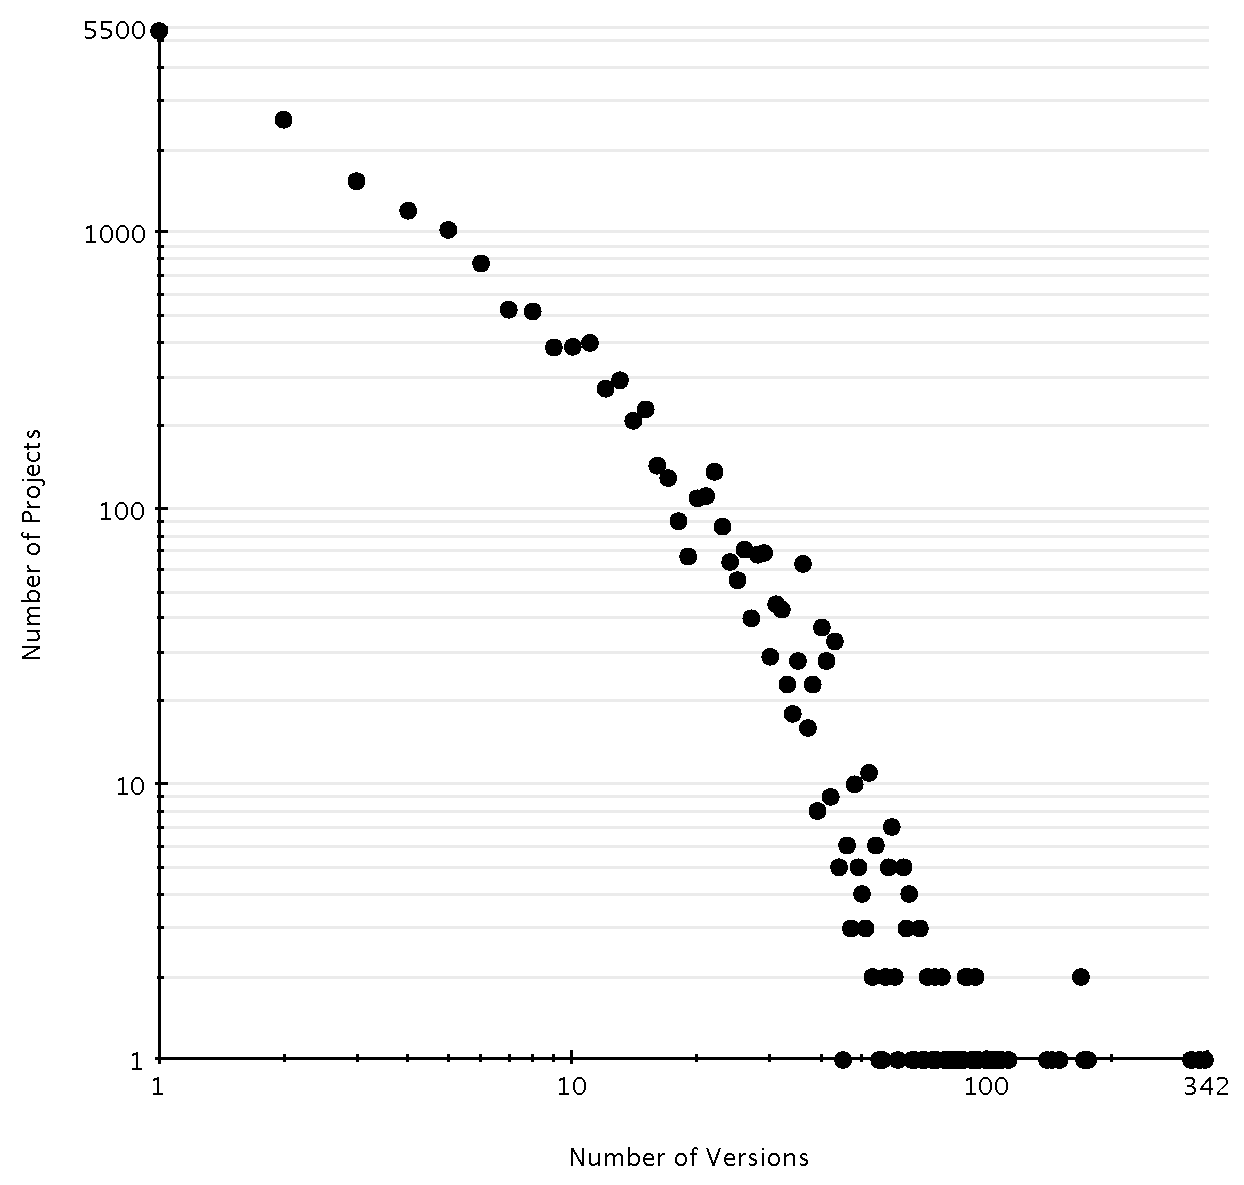
\includegraphics[scale=0.6]{version_count.pdf}
\end{figure*}

\begin{table}
\centering
\caption{Descriptive Statistics Measurements for the Maven Repository}
\label{tbl:repository}
\begin{tabular}{l r}
 \hline
Projects & 17,505\\
Versions (total) & 114,399\\
Min & 1\\
Max & 337\\
Mean & 6.54\\
Median & 3\\
Range & 336\\
1$^{st}$ Quartile & 1\\
3$^{rd}$ Quartile & 8\\
\hline
\end{tabular}
\end{table}

\subsection{Experiment}
\label{sec:exp}

\section{Results and Analysis}
\label{sec:res}

\section{Related Work}
\label{sec:rel}

There are noumerous methods for mining software repositories in the context
of software evolution~\cite{KCM07}. In this section we focus on the ones
that highlight the relationship between software bugs and evolution and try to
extract useful conclusions. The key idea behind this concept is
similar to ours: the combination of information like bug decriptions,
documentation and others with the information retrieved from either the source
or object code of a project version.

{\it Refactoring identification} through software evolution is an approach used to
relate refactorings with software bugs. Wei{\ss}gerber et al. found that a high
ratio of refactorings is usually followed by an increasing ratio of bug
reports~\cite{WD06}. In addition, they indicated that software bugs are sometimes introduced
after an incomplete refactoring~\cite{GW05}.
Ratzinger et al.~\cite{RSG08} showed that the number of bugs decreases, when the number of
refactorings increases. Finally, Kim M. et al.~\cite{KCK11} indicated that {\sc api}-level
refactorings aid bug fixes.

Using {\it micro patterns} is a method proposed by Kim et al.~\cite{KPW06}
to detect bug-prone patterns among source code. Micro patterns describe programming
idioms like inheritance, data management, immutability and others. The approach involved
the examination of all revisions of three open-source projects to extract bug
introduction rates for each pattern. Gil et al.~\cite{GM05} analyzed the
prevalence of micro patterns across five Sun {\sc jdk} versions to conclude that
pattern prevalence tends to be the same in software collections.

{\it Querying techniques} are used to answer a broad range of questions
regarding the evolution history of a project~\cite{HG05}. Bhattacharya et
al.~\cite{BN11, B11} proposed a framework that is based upon
recursively enumerable languages. The framework can correlate software
bugs with developers in various ways. For instanse, return the list of
bugs fixed by a specific developer. Fischer et al.~\cite{FPG03} proposed
an approach for populating a release history database that combines code
information with bug tracking data. In this way, a developer can couple files
that contain common bugs, estimate code maturity with respect to the bugs
and others. The ``Ultimate Debian Database''~\cite{NZ10} is an {\sc sql}-based
framework that integrates information about the Debian project from various
sources to answer queries related to software bugs and source code.

D'Ambros et al. have used {\it bug history analysis} to detect
the critical components of a project~\cite{D08}. This is done by using an
evolutionary meta-model~\cite{DL08}. The same approach was
also used by Zimmermann et al.~\cite{ZNA08} to check the correlation
of bugs with software properties like code complexity, process quality and others
and predict future properties.

Contrary to the above, our work focuses on the subset of security bugs.
Focusing on such bugs is not a new idea. Massacci et al.~\cite{MNN11} observed
the evolution of software defects by examining six major versions of Firefox.
To achieve this they created a database schema that contained information
coming from the ``Mozilla Firefox-related Security Advisories'' ({\sc mfsa})
list,~\footnote{\url{http://www.mozilla.org/projects/security/known-vulnerabilities.html}}
Bugzilla entries and others. Their findings indicated that security bugs are
persistent over time. They also showed that there are many web users that use
old versions of Firefox, meaning that old attacks will continue to work.
Zaman et al.~\cite{ZAH11} focused again on Firefox to study the relation of
security bugs with performance bugs. This was also done by analyzing the project's
Bugzilla. Their research showed that security bugs require more experienced developers
to be fixed. In addittion, security bug fixes are more complex than the
fixes of performance and other bugs.
Shahzad et al.~\cite{SSL12} analyzed large sets of vulnerability data-sets to observe
various features of the vulnerabilities that they considered critical. Such features
were the functionality and the criticality of the defects. Their analysis
included the observation of vulnerability disclosures, the behavior of
hackers in releasing exploits for vulnerabilities, patching and others. In
their findings they highlighted the most exploited defects and showed that
the percentage of remotely exploitable vulnerabilities has gradually increased
over the years.

\section{Conclusions and Future Work}
\label{sec:con}

Our work could (?) aid bug-prediction models in the same way as~\cite{BN11}.

\section*{Acknowledgments}

The project is being co-financed by the European Regional Development Fund (ERDF)
and national funds and is a part of the Operational Programme ``Competitiveness \&
Entrepreneurship" (OPCE II), Measure ``COOPERATION" (Action I).

\bibliographystyle{IEEEtran}
\bibliography{msr} 

\end{document}


